\documentclass[border=6pt]{standalone}
\usepackage{amsmath,amssymb}
\usepackage{tikz}
\usetikzlibrary{arrows.meta,positioning,shadows,calc}
\begin{document}
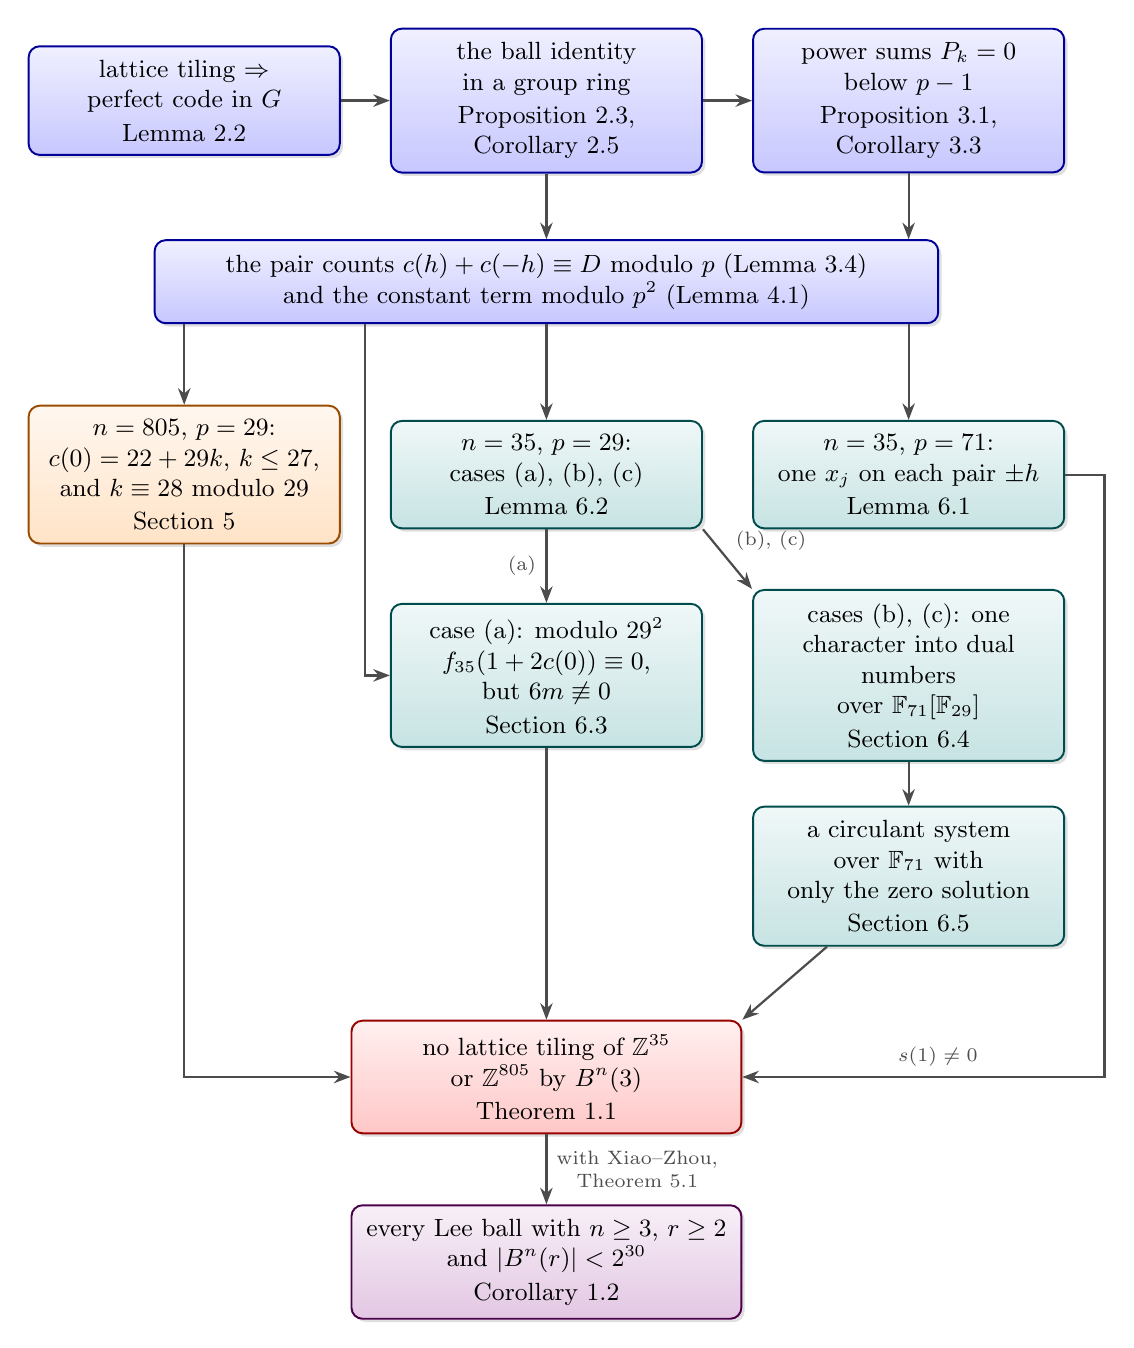
\begin{tikzpicture}[
  box/.style={draw=#1!60!black,line width=0.7pt,rounded corners=4pt,
    top color=#1!6,bottom color=#1!22,drop shadow={opacity=0.25,shadow xshift=1.2pt,shadow yshift=-1.2pt},
    align=flush center,font=\small,inner sep=5pt,minimum height=1.3cm,text width=3.6cm},
  arr/.style={-{Stealth[length=6pt]},line width=0.8pt,black!70},
  lab/.style={font=\scriptsize,align=flush center,black!70}]
% the general tools
\node[box=blue] (red) at (0,0) {lattice tiling $\Rightarrow$\\ perfect code in $G$\\[1pt] Lemma 2.2};
\node[box=blue] (ball) at (4.6,0) {the ball identity\\ in a group ring\\[1pt] Proposition 2.3, Corollary 2.5};
\node[box=blue] (mom) at (9.2,0) {power sums $P_k=0$\\ below $p-1$\\[1pt] Proposition 3.1, Corollary 3.3};
\node[box=blue,text width=9.6cm,minimum height=1.05cm] (tools) at (4.6,-2.3)
  {the pair counts $c(h)+c(-h)\equiv D$ modulo $p$ (Lemma 3.4)\\ and the constant term modulo $p^2$ (Lemma 4.1)};
% n = 805
\node[box=orange] (n805) at (0,-4.75) {$n=805$, $p=29$:\\ $c(0)=22+29k$, $k\le27$,\\ and $k\equiv28$ modulo $29$\\[1pt] Section 5};
% n = 35
\node[box=teal] (l29) at (4.6,-4.75) {$n=35$, $p=29$:\\ cases (a), (b), (c)\\[1pt] Lemma 6.2};
\node[box=teal] (l71) at (9.2,-4.75) {$n=35$, $p=71$:\\ one $x_j$ on each pair $\pm h$\\[1pt] Lemma 6.1};
\node[box=teal] (casea) at (4.6,-7.3) {case (a): modulo $29^2$\\ $f_{35}(1+2c(0))\equiv0$,\\ but $6m\not\equiv0$\\[1pt] Section 6.3};
\node[box=teal] (joint) at (9.2,-7.3) {cases (b), (c): one\\ character into dual numbers\\ over $\mathbb F_{71}[\mathbb F_{29}]$\\[1pt] Section 6.4};
\node[box=teal] (circ) at (9.2,-9.85) {a circulant system\\ over $\mathbb F_{71}$ with\\ only the zero solution\\[1pt] Section 6.5};
\node[box=red,text width=4.6cm] (main) at (4.6,-12.4) {no lattice tiling of $\mathbb Z^{35}$\\ or $\mathbb Z^{805}$ by $B^n(3)$\\[1pt] Theorem 1.1};
\node[box=violet,text width=4.6cm] (cor) at (4.6,-14.75) {every Lee ball with $n\ge3$, $r\ge2$\\ and $|B^n(r)|<2^{30}$\\[1pt] Corollary 1.2};
% arrows
\draw[arr] (red) -- (ball);
\draw[arr] (ball) -- (mom);
\draw[arr] (ball.south) -- (ball.south |- tools.north);
\draw[arr] (mom.south) -- (mom.south |- tools.north);
\draw[arr] (tools.south -| n805.north) -- (n805.north);
\draw[arr] (tools.south -| l29.north) -- (l29.north);
\draw[arr] (tools.south -| l71.north) -- (l71.north);
\draw[arr] (tools.south -| 2.3,0) -- (2.3,-7.3) -- (casea.west);
\draw[arr] (l29) -- node[lab,left]{(a)} (casea);
\draw[arr] (l29.south east) -- node[lab,above right=-1pt]{(b), (c)} (joint.north west);
\draw[arr] (joint) -- (circ);
\draw[arr] (circ) -- (main.north east);
\draw[arr] (casea) -- (main);
\draw[arr] (n805.south) |- (main.west);
\draw[arr] (l71.east) -- ++(0.5,0) |- node[lab,pos=0.73,above]{$s(1)\ne0$} (main.east);
\draw[arr] (main) -- node[lab,right]{with Xiao--Zhou,\\ Theorem 5.1} (cor);
\end{tikzpicture}
\end{document}
